\section{Schlaganfall}

Jährlich erleiden rund 15 Millionen Menschen weltweit einen Schlaganfall, von denen \ac{ca.} 5 Millionen Betroffene sterben und weitere 5 Millionen bleibende Schäden davontragen (siehe Abbildung \ref{fig:stroke_burden}). \cite{atlas:2004:mackay} 

\begin{figure}[H]
    \centering
    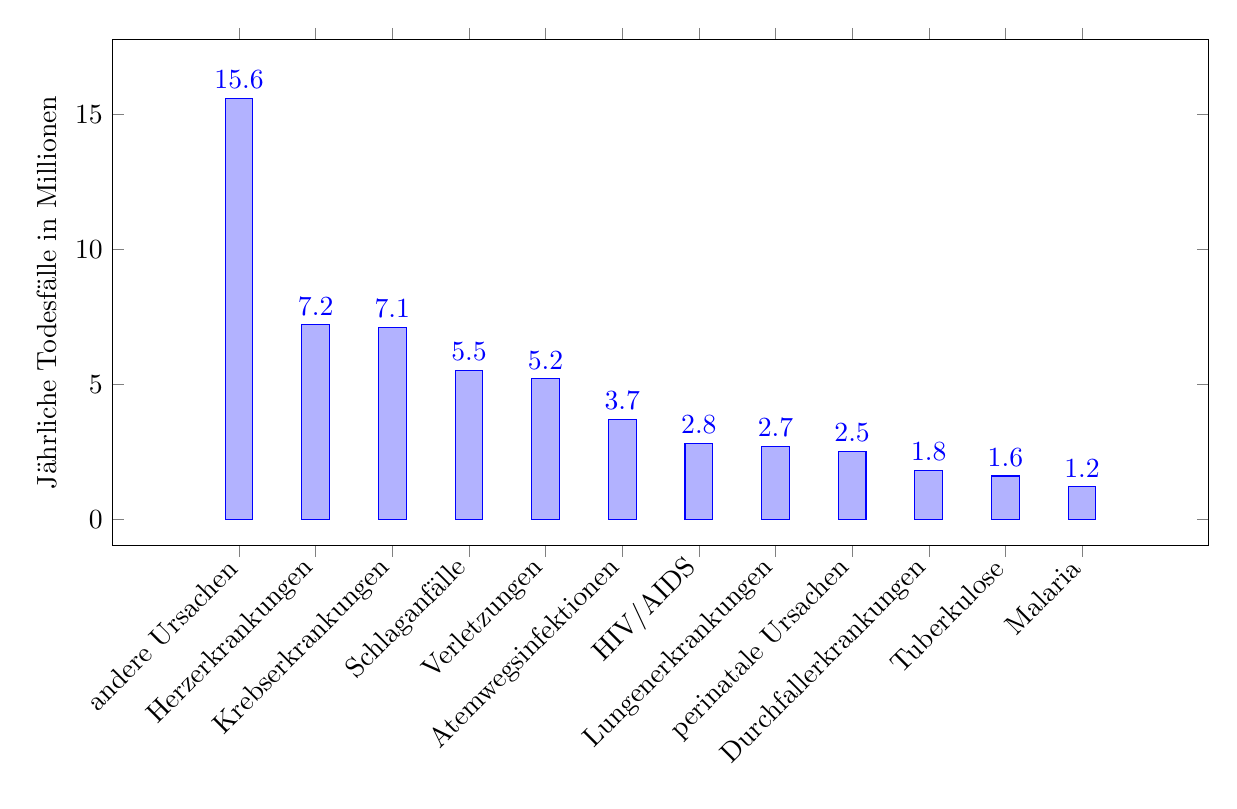
\begin{tikzpicture}
        \begin{axis}[
            ybar, height=8cm, width=15.5cm,
            enlargelimits=0.15,
            legend style={at={(0.5,-0.15)},
              anchor=north,legend columns=-1},
            ylabel={Jährliche Todesfälle in Millionen},
            symbolic x coords={andere Ursachen, Herzerkrankungen, Krebserkrankungen, Schlaganfälle, Verletzungen, Atemwegsinfektionen, HIV/AIDS, Lungenerkrankungen, perinatale Ursachen, Durchfallerkrankungen, Tuberkulose, Malaria},
            xtick=data,
            nodes near coords,
            nodes near coords align={vertical},
            x tick label style={rotate=45,anchor=east}
            ]
        \addplot coordinates {
            (andere Ursachen, 15.6) 
            (Herzerkrankungen, 7.2) 
            (Krebserkrankungen, 7.1)
            (Schlaganfälle, 5.5)
            (Verletzungen, 5.2)
            (Atemwegsinfektionen, 3.7)
            (HIV/AIDS, 2.8)
            (Lungenerkrankungen, 2.7)
            (perinatale Ursachen, 2.5)
            (Durchfallerkrankungen, 1.8)
            (Tuberkulose, 1.6)
            (Malaria, 1.2)
            };
        \end{axis}
    \end{tikzpicture}
    \caption{Schlaganfall im Vergleich mit anderen Todesursachen \cite{atlas:2004:mackay}.}
    \label{fig:stroke_burden}
\end{figure}

Nach Herzerkrankungen und Krebserkrankungen befindet sich der Schlaganfall in der Liste der häufigsten Todesursachen der Welt auf Platz 3. Die Gefahr einen Schlaganfall zu erleiden, steigt mit dem Alter an. Ab 55 verdoppelt sich die Erkrankungsrate mit jedem zusätzlichen Lebensjahrzehnt. Trotzdem sind junge Menschen nicht davor geschützt, denn 6\% der Erkrankten sind unter 45. Ein Schlaganfall wird durch eine Verstopfung oder das plötzliche Platzen einer Gehirnarterie, welche eine Durchblutungsstörung im Gehirn hervorruft, ausgelöst (siehe Abbildung \ref{fig:stroke_cause}). Betroffene Hirnareale werden nicht mehr ausreichend mit Sauerstoff versorgt und sterben deswegen ab. Das Zeitfenster für eine erfolgreiche Behandlung ist mit maximal 4,5 Stunden sehr gering. Grundsätzlich werden vier unterschiedliche Formen von Schlaganfällen unterschieden, jedoch zählen der \nameref{paragrah:isch_insult} (80\% Häufigkeit) und der \nameref{paragrah:isch_haemor} oder Gehirnblutung (15\% Häufigkeit) zu den häufigsten Arten. Weniger verbreitet sind die Sinusvenenthrombose (5\% Häufigkeit) und das sogenannte \enquote{Schlagerl}. Die Indizien für einen Schlaganfall können ganz plötzlich auftreten und sind auf einen Nährstoffmangel im Gehirn zurückzuführen. Die Symptomatik ist von der Lokalisation abhängig. Zu den häufigsten Indizien für einen Insult zählen Bewegungsstörungen, Empfindungsstörungen, Sprachstörungen, Sehstörungen, Koordinationsstörungen und Gangunsicherheit. Am häufigsten zeigt sich eine Kombination aus verschiedenen Symptomen, wie Sprach- oder Sehstörung, halbseitige Lähmung oder Taubheitsgefühl. \cite{haring:2014:insult}

\begin{figure}[h]
    \centering
	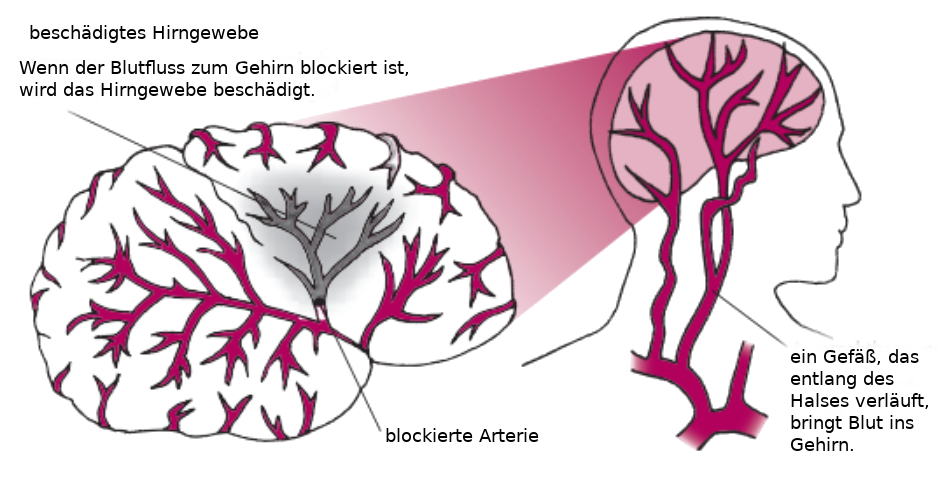
\includegraphics[width=1\linewidth]{figures/stroke/stroke_cause_deu}
	\caption{Ein Schlaganfall tritt auf, wenn die Blutzufuhr zum Gehirn unterbrochen wird. (aus dem Englischen nach \cite{world:2005:avoiding})}
	\label{fig:stroke_cause}
\end{figure}

\paragraph{Ischämischer Insult} \label{paragrah:isch_insult} 
Ursache eines Ischämischen Insults ist ein Blutgerinnsel, welches eine Gehirnarterie verstopft und damit den Blutfluss zum Gehirn blockiert. Hirninfakt ist eine weitere Bezeichnung für diesen Typ Schlaganfall, da jener das Gegenstück zum Herzinfakt darstellt. \cite{haring:2014:insult} 

\paragraph{Hämorrhagischer Schlaganfall}\label{paragrah:isch_haemor} 
Auslöser eines solchen Schlaganfalls ist eine geplatzte Arterie im Gehirn. Wenn eine Gehirnarterie zerreißt, dann tritt Blut mit hohem Druck in das Gehirngewebe ein. Wenn jedoch nur ein \Gls{aneurysma} platzt, dann bleibt die Blutung an der Gehirnoberfläche. \cite{haring:2014:insult} 

\subsection{Ursachen}
Zu den Auslösern von Schlaganfällen zählen Bluthochdruck, hohe Blutfettwerte, Rauchen, Mangel an Bewegung oder hormonelle Einflüsse \cite{haring:2014:insult}\cite{world:2005:avoiding}. Aber auch Krankheiten wie Atherosklerose, Diabetes mellitus (Zuckerkrankheit), Vorhofflimmern, Tumore oder rheumatische Erkrankungen können Risikofaktoren sein. \cite{haring:2014:insult} 

\subsection{Folgen}
Die Folgeschäden eines Schlaganfalls unterscheiden sich von Person zu Person, je nach Typ, Schweregrad, Lokalisation und Anzahl der Schlaganfälle. Wenn ein Bereich des Gehirns durch einen Schlaganfall beschädigt wird, dann kann der Verlust von diversen Körperfunktionen die Folge sein. Jeder Bereich des Gehirns ist für eine Funktion oder Fähigkeit zuständig. Das menschliche Gehirn unterteilt sich in drei Hauptbereiche (siehe Abbildung \ref{fig:brain_areas}): \cite{hopkins:2019:stroke_effects}

\begin{itemize}
    \item \textbf{Großhirn}: Zuständig für Bewegung, Empfindung, Sprache, logisches Denken, Gedächtnis, Sehvermögen und Emotionen.
    \item \textbf{Kleinhirn}: Unterstützt Koordinierung von Muskeln, Feinbewegungen, Koordination und Gleichgewicht.
    \item \textbf{Hirnstamm}: Steuert viele lebenswichtige Funktionen, wie Herzschlag, Blutdruck und Atmung. Außerdem hilft der Hirnstamm bei der Kontrolle von Hauptnerven wie Augen, Ohren, Sprache, Kauen und Schlucken.
\end{itemize}

Je nachdem, wo der Schlaganfall auftritt, unterscheiden sich die Auswirkungen der Krankheit deutlich. \cite{hopkins:2019:stroke_effects} 

\begin{figure}[h]
    \centering
	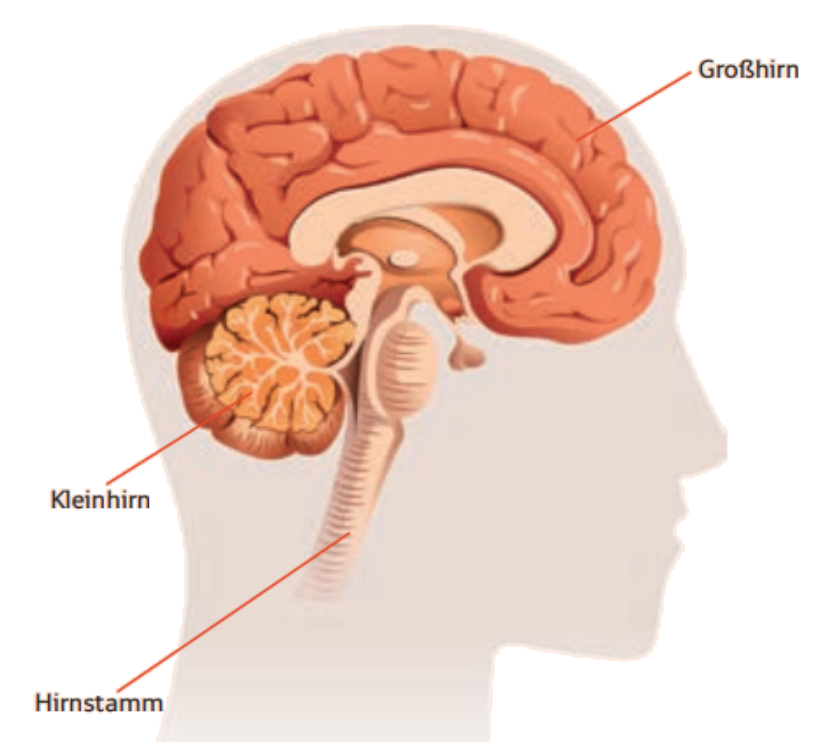
\includegraphics[width=0.5\linewidth]{figures/stroke/brain_areas}
	\caption{Die drei Hauptteile des Gehirns. \cite{haring:2014:insult}}
	\label{fig:brain_areas}
\end{figure}

Die Behandlung eines Schlaganfalls muss so schnell wie möglich erfolgen, da pro Minute rund zwei Millionen Nervenzellen zerstört werden \cite{haring:2014:insult}. Je nach Stärke der Hirnschädigung ist der/die Betroffene mehr oder weniger stark in körperlicher und geistiger Leistungsfähigkeit eingeschränkt. Oftmals sind Teile des Körpers nur noch beeinträchtigt nutzbar. Eine einseitige Lähmung (Hemiparese) kann einen Arm, die Hand, ein Bein, aber auch eine gesamte Körperhälfte (Hemiplegie) betreffen. Hinzukommend können häufig Sprach-, Sehstörungen oder Schluckbeschwerden vorliegen. Außerdem können Bewusstseins- und Wahrnehmungsstörungen als Folge auftreten. \cite{health:2019:stroke_rehab}\cite{stroke:2019:consequences} \\ 
Ein Schlaganfall bringt häufig psychische Probleme mit sich. Vielfach handelt es sich um Depressionen, in diesem Fall wird es eine Post-Stroke-Depression genannt. Drei Monate nach dem Ausbrechen der Krankheit haben bereits 20\% aller Patient/innen eine depressive Störung. \cite{haring:2014:insult}

\subsection{Rehabilitation}
Die Rehabilitation nach einem Schlaganfall hat das Ziel, den/die Patient/in zurück in den Alltag zu bringen. Die Funktionen, die durch den Insult beschädigt wurden, sollen größtmöglich wiederhergestellt werden und den Betroffenen soll der Wiedereinstieg in ein selbstständiges Leben ermöglicht werden. Ein möglichst früher Beginn der Rehabilitation kann die Folgeschäden nicht gänzlich verhindern, jedoch reduzieren. Für eine erfolgreiche Therapie ist eine Vielzahl von Expert/innen notwendig. Diese Fachkräfte kommen aus den Bereichen der Physiotherapie, Ergotherapie, Logopädie und Neuropsychologie. Um das Wohlbefinden der Patient/innen kümmern sich Ärzt/innen und Pflegekräfte. Tote Gehirnzellen können nicht ersetzt werden, jedoch sind benachbarte Regionen in der Lage, Funktionen auszugleichen oder zu übernehmen. Durch physiotherapeutische oder logopädische Maßnahmen können Handlungen wieder neu erlernt werden. Die Therapeut/innen entwickeln gemeinsam mit den Patient/innen Ziele, die in kurzer Zeit erreichbar sind. Die Übungen sind stets auf die Wünsche und Bedürfnisse des/der Behandelten ausgelegt. Jemand, der zu viel auf einmal erreichen will, wird schnell enttäuscht werden und die Motivation sinkt. Kleinste Fortschritte sollen von den Angehörigen und den Patient/innen positiv bewertet werden. \cite{haring:2014:insult}

Verteilung der Aufgaben in der Rehabilitation: \cite{haring:2014:insult}
\begin{itemize}
    \item \textbf{Neuropsychologie}: Ein/e Neuropsycholog/in untersucht den/die Patient/in auf seine/ihre geistigen Funktionseinschränkungen. Das Training der Aufmerksamkeit, Merkfähigkeit und Konzentration wird ebenfalls durch eine/n Expert/in der Neuropsychologie übernommen. Die jeweilige Fachkraft ist außerdem für die psychologische Betreuung der Angehörigen zuständig.
    
    \item \textbf{Physiotherapie}: Die Hauptaufgabe der Physiotherapie ist die Wiederherstellung der verloren gegangen motorischen Körperfunktionen. Es werden Gleichgewicht, Gangsicherheit und Kraft trainiert. Des Weiteren fällt die Vermeidung von Stürzen und die Vorbeugung von falschen Bewegungsmustern unter den Aufgabenbereich des/der Physiotherapeut/in.
    
    \item \textbf{Ergotherapie}: Hauptziel des/der Ergotherapeut/in ist die Unterstützung des/der Patient/in bei der Wiedereingliederung in den Alltag. Der/die Betroffene soll alltägliche Aufgaben, wie das selbständige Anziehen, Waschen \ac{usw.} wieder beherrschen. Aufgrund der Wichtigkeit der Greifbewegung im Alltag liegt der Fokus der Ergotherapie auf den verschiedenen Armfunktionen. Den Betroffenen wird gezeigt, wie sie trotz Behinderung, alltägliche Aufgaben meistern.
    
    \item \textbf{Logopädie}: Eine Behandlung durch eine/n Logopäd/in kommt bei Sprach-, Sprech- und Schluckstörungen zum Einsatz. Sprachstörungen bezeichnen eine Beeinträchtigung des Sprachverständnisses. Bei Sprechstörungen sind Worte aufgrund der nicht funktionalen Sprechmotorik unverständlich. In der Logopädie trainieren Therapeut/innen häufig das Nachsprechen und Vervollständigen von diversen Begriffen.
\end{itemize}



